% =====================================================================
\chapter{Kết quả nghiên cứu}
\label{chap:ketqua}

Chương này trình bày kết quả theo thứ tự của ba câu hỏi nghiên cứu. Mục~\ref{sec:res-fs} báo cáo kết quả học có giám sát, làm bối cảnh để đọc các kết quả còn lại. Mục~\ref{sec:res-rq1} trả lời CH1 bằng cách so sánh DACL với tám phương pháp bán giám sát và với học có giám sát. Mục~\ref{sec:res-rq2} và~\ref{sec:res-qual} trả lời CH2, lần lượt bằng phân tích định lượng về loại lỗi và độ khó của ảnh, và bằng quan sát định tính. Mục~\ref{sec:res-dynamics} trình bày diễn biến huấn luyện của DACL, bổ sung bằng chứng thực nghiệm cho CH3. Người đọc chỉ cần các kết luận có thể chuyển thẳng sang Chương~\ref{chap:ketluan}. Mọi con số trong chương được tính từ các tệp kết quả lưu trong thư mục \texttt{results/} của kho mã nguồn.

\section{Kết quả học có giám sát}
\label{sec:res-fs}

Bảng~\ref{tab:fs} cho thấy khi số ảnh có nhãn tăng từ 5\% (46 ảnh) lên 100\% (930 ảnh), DSC của UNeXt chỉ tăng từ 94,15\% lên 95,23\%, tức là 1,08 điểm. Với Swin-Unet, mức tăng là 0,73 điểm. Như vậy, trên bộ dữ liệu này và ở độ phân giải $224\times224$, chỉ 46 ảnh có nhãn đã đủ để đạt phần lớn độ chính xác có thể đạt được. Dư địa mà học bán giám sát có thể cải thiện so với học có giám sát trên cùng số nhãn chỉ khoảng một điểm DSC.

\begin{table}[ht]
\centering
\caption{Kết quả học có giám sát trên tập kiểm thử theo tỷ lệ ảnh có nhãn. DSC và Jaccard tính bằng \%, HD95 và ASD tính bằng điểm ảnh ở độ phân giải $224\times224$.}
\label{tab:fs}
\small
\begin{tabular}{llcccc}
\toprule
Mạng & Nhãn & DSC $\uparrow$ & Jaccard $\uparrow$ & HD95 $\downarrow$ & ASD $\downarrow$ \\
\midrule
\inputtable{tables/fs.tex}
\bottomrule
\end{tabular}
\end{table}

Swin-Unet cao hơn UNeXt ở mọi mức nhãn, từ 0,10 đến 0,57 điểm DSC, và khoảng cách lớn nhất ở mức 5\% nhãn. Đây là khoảng cách mà DACL hướng tới thu hẹp: đưa UNeXt đến gần độ chính xác của Swin-Unet, trong khi chi phí suy luận chỉ bằng khoảng một phần bảy (Bảng~\ref{tab:complexity}).

\section{Độ chính xác của DACL so với các phương pháp khác (CH1)}
\label{sec:res-rq1}

Bảng~\ref{tab:ssl5} và~\ref{tab:ssl10} trình bày kết quả của mười một mô hình ở mức 5\% và 10\% nhãn. Cột $p$ là kết quả kiểm định Wilcoxon theo cặp trên DSC của từng ảnh, so với DACL.

\begin{table}[p]
\centering
\caption{Kết quả trên tập kiểm thử với 5\% ảnh có nhãn. DSC và Jaccard tính bằng \%, HD95 và ASD tính bằng điểm ảnh ở độ phân giải $224\times224$. Trong nhóm bán giám sát, giá trị tốt nhất được \textbf{in đậm} và tốt thứ hai được \textit{in nghiêng}. Cột $p$: kiểm định Wilcoxon theo cặp trên DSC của từng ảnh so với DACL; ngưỡng ý nghĩa sau hiệu chỉnh Bonferroni là 0,005.}
\label{tab:ssl5}
\resizebox{\textwidth}{!}{%
\begin{tabular}{lcccccccc}
\toprule
Phương pháp & Có nhãn & Không nhãn & DSC $\uparrow$ & Jaccard $\uparrow$ & HD95 $\downarrow$ & ASD $\downarrow$ & $p$ \\
\midrule
\inputtable{tables/ssl_5.tex}
\bottomrule
\end{tabular}}
\end{table}

\begin{table}[p]
\centering
\caption{Kết quả trên tập kiểm thử với 10\% ảnh có nhãn. Quy ước như Bảng~\ref{tab:ssl5}.}
\label{tab:ssl10}
\resizebox{\textwidth}{!}{%
\begin{tabular}{lcccccccc}
\toprule
Phương pháp & Có nhãn & Không nhãn & DSC $\uparrow$ & Jaccard $\uparrow$ & HD95 $\downarrow$ & ASD $\downarrow$ & $p$ \\
\midrule
\inputtable{tables/ssl_10.tex}
\bottomrule
\end{tabular}}
\end{table}

\subsection{Độ trùng khớp}

Ở cả hai mức nhãn, DACL có DSC và Jaccard cao nhất trong nhóm bán giám sát. Ở mức 5\%, DACL đạt DSC 94,38\%, hơn phương pháp đứng thứ hai là PCPCS 0,39 điểm và hơn MT 1,21 điểm. Ở mức 10\%, DACL đạt 94,46\%, hơn DSTCT, phương pháp đứng thứ hai, 0,60 điểm. Khác biệt giữa DACL và từng phương pháp bán giám sát đều có ý nghĩa thống kê sau hiệu chỉnh Bonferroni ($p<0{,}001$). Xét riêng nhóm CNN--Transformer, DACL hơn LMCT 0,64 điểm ở mức 5\% và 0,92 điểm ở mức 10\%.

So với học có giám sát trên cùng số ảnh có nhãn, kết quả khác đi. Ở mức 5\%, DACL cao hơn UNeXt học có giám sát 0,23 điểm, nhưng khác biệt không có ý nghĩa thống kê ($p=0{,}073$). Ở mức 10\%, DACL thấp hơn 0,14 điểm, và khác biệt có ý nghĩa ($p<0{,}001$). Tám phương pháp đối chứng đều thấp hơn UNeXt học có giám sát ở cả hai mức. DACL là phương pháp bán giám sát duy nhất không thua kém có ý nghĩa ở mức 5\%. Swin-Unet học có giám sát cao hơn DACL 0,34 điểm ở mức 5\% và 0,55 điểm ở mức 10\%.

\subsection{Độ chính xác biên}

Về biên, DACL không giữ được vị trí dẫn đầu. HD95 của DACL ở mức 5\% là 3,01 điểm ảnh, đứng thứ tám trong chín phương pháp bán giám sát, chỉ trên DSTCT. Kiểm định Wilcoxon với hiệu chỉnh Bonferroni cho thấy ICT, MT, DCT và CPS có HD95 thấp hơn DACL một cách có ý nghĩa, với mức chênh 0,12--0,20 điểm ảnh. Ở mức 10\%, HD95 của DACL (2,97) đứng thứ sáu, và MT, PCPCS, DCT, CTCT thấp hơn có ý nghĩa. Ngược lại, ASD của DACL thuộc nhóm tốt nhất: thứ hai ở mức 5\% (0,81, sau CPS với 0,80) và tốt nhất ở mức 10\% (0,80). Hai độ đo biên cho kết quả khác nhau vì ASD là trung bình khoảng cách trên mọi điểm biên, còn HD95 bị chi phối bởi 5\% điểm biên xa nhất. Kết quả này gợi ý rằng DACL khớp biên tốt ở phần lớn tế bào, nhưng sinh ra một số vùng sai lệch nằm xa tế bào thật. Các mức chênh 0,1--0,2 điểm ảnh ở độ phân giải $224\times224$ đều rất nhỏ so với kích thước một tế bào.

\subsection{Ảnh hưởng của số lượng nhãn}

Khi tăng từ 5\% lên 10\% nhãn, DSC của DACL tăng 0,08 điểm, còn của UNeXt học có giám sát tăng 0,45 điểm. Một số phương pháp đối chứng lại giảm: CPS giảm 0,87, PCPCS giảm 0,36, DCT giảm 0,35 và LMCT giảm 0,20 điểm. Nhân đôi số ảnh có nhãn về lý thuyết không nên làm mô hình kém đi. Vì vậy, các mức giảm này nhiều khả năng phản ánh dao động giữa các lần huấn luyện, do mỗi cấu hình chỉ được chạy một lần. Biên độ của dao động, có trường hợp gần 0,9 điểm, cùng bậc với khoảng cách giữa các phương pháp đối chứng. Ngược lại, vị trí dẫn đầu của DACL được lặp lại ở cả hai mức nhãn, với khoảng cách 0,39--0,60 điểm so với phương pháp thứ hai.

\section{Loại lỗi và độ khó của ảnh (CH2): kết quả định lượng}
\label{sec:res-rq2}

\subsection{Độ chính xác và độ phủ}

Toàn bộ 22 mô hình được chạy lại trên tập kiểm thử. DSC tính lại khớp với kết quả lưu khi huấn luyện đến hai chữ số thập phân. Bảng~\ref{tab:precrec} trình bày precision, recall và tỷ lệ diện tích dự đoán so với mặt nạ chuẩn.

\begin{table}[ht]
\centering
\caption{Độ chính xác, độ phủ (\%) và tỷ lệ diện tích dự đoán so với mặt nạ chuẩn, lấy trung bình trên 265 ảnh kiểm thử.}
\label{tab:precrec}
\small
\begin{tabular}{lcccccc}
\toprule
 & \multicolumn{3}{c}{5\% nhãn} & \multicolumn{3}{c}{10\% nhãn} \\
\cmidrule(lr){2-4}\cmidrule(lr){5-7}
Phương pháp & Precision & Recall & Diện tích & Precision & Recall & Diện tích \\
\midrule
\inputtable{tables/precrec.tex}
\bottomrule
\end{tabular}
\end{table}

Bảng~\ref{tab:precrec} cho ba kết quả. Thứ nhất, mọi mô hình, kể cả hai mô hình học có giám sát, đều dự đoán diện tích lớn hơn mặt nạ chuẩn từ 2\% đến 6\%. Thứ hai, tất cả các phương pháp bán giám sát đều có precision thấp hơn UNeXt học có giám sát, tức là sinh ra nhiều dương tính giả hơn. Thứ ba, DACL có precision cao nhất trong nhóm bán giám sát ở cả hai mức nhãn. Recall của DACL cũng cao nhất ở mức 5\%, và chỉ thấp hơn LMCT ở mức 10\%. LMCT đạt recall cao nhờ dự đoán lấn biên nhiều nhất: diện tích lớn hơn mặt nạ chuẩn 6\%, kéo theo precision thấp nhất. Ưu thế DSC của DACL vì vậy đến từ việc giảm đồng thời cả hai loại lỗi so với các phương pháp bán giám sát khác, chứ không phải từ việc đánh đổi loại lỗi này lấy loại lỗi kia.

\subsection{Phân bố lợi ích theo độ khó của ảnh}

Ở mức 5\% nhãn, DSC trung bình của DACL cao hơn UNeXt học có giám sát, nhưng DACL chỉ tốt hơn trên 98 trong 265 ảnh. Trung vị của hiệu DSC giữa hai mô hình là $-0{,}12$ điểm. Bảng~\ref{tab:quartile} chia ảnh kiểm thử thành bốn nhóm theo tứ phân vị DSC của UNeXt học có giám sát, từ nhóm khó nhất (Q1) đến nhóm dễ nhất (Q4).

\begin{table}[ht]
\centering
\caption{Hiệu DSC trung bình (điểm \%) so với UNeXt học có giám sát, theo nhóm tứ phân vị độ khó. Mỗi nhóm có 66 hoặc 67 ảnh.}
\label{tab:quartile}
\small
\begin{tabular}{lccc ccc}
\toprule
 & \multicolumn{3}{c}{5\% nhãn} & \multicolumn{3}{c}{10\% nhãn} \\
\cmidrule(lr){2-4}\cmidrule(lr){5-7}
Nhóm & DACL & CPS & FS Swin-Unet & DACL & CPS & FS Swin-Unet \\
\midrule
Q1 (khó nhất) & $+1{,}42$ & $+0{,}31$ & $+1{,}31$ & $+0{,}34$ & $-1{,}03$ & $+0{,}90$ \\
Q2            & $-0{,}01$ & $-0{,}25$ & $+0{,}35$ & $-0{,}12$ & $-1{,}30$ & $+0{,}29$ \\
Q3            & $-0{,}16$ & $-0{,}36$ & $+0{,}41$ & $-0{,}27$ & $-1{,}64$ & $+0{,}29$ \\
Q4 (dễ nhất)  & $-0{,}31$ & $-0{,}39$ & $+0{,}21$ & $-0{,}48$ & $-1{,}96$ & $+0{,}17$ \\
\bottomrule
\end{tabular}
\end{table}

Ở mức 5\%, DACL cải thiện trung bình 1,42 điểm trên nhóm khó nhất. Riêng 20 ảnh mà UNeXt học có giám sát đạt DSC dưới 90\%, mức cải thiện là 3,75 điểm. Ngược lại, DACL kém hơn một chút trên ba nhóm còn lại, và mức kém lớn nhất ($-0{,}31$) rơi vào nhóm dễ nhất. Mức 10\% có cùng xu hướng nhưng yếu hơn: $+0{,}34$ ở Q1 và $-0{,}48$ ở Q4. Vì các nhóm được xác định theo chính điểm số của UNeXt học có giám sát, nhóm Q1 chứa cả những ảnh mà mô hình này kém do ngẫu nhiên. Bất kỳ mô hình nào khác cũng có xu hướng tốt hơn ở nhóm đó, theo hiện tượng hồi quy về trung bình. Cột Swin-Unet học có giám sát phản ánh rõ hiệu ứng này. Điểm phân biệt DACL nằm ở hai đầu bảng. Ở Q1, mức cải thiện của DACL tương đương Swin-Unet học có giám sát, một mạng lớn gấp 17 lần. Ở Q4, DACL lại kém UNeXt học có giám sát, trong khi Swin-Unet vẫn tốt hơn. CPS, chỉ giám sát chéo giữa hai mạng UNeXt mà không có Swin-Unet và $\Ldac$, có mức cải thiện ở Q1 thấp hơn nhiều.

\section{Loại lỗi và độ khó của ảnh (CH2): kết quả định tính}
\label{sec:res-qual}

Hình~\ref{fig:qual} so sánh dự đoán của UNeXt học có giám sát và năm phương pháp bán giám sát gần đây nhất ở mức 5\% nhãn, trên bốn ảnh kiểm thử được chọn theo tiêu chí ở mục~\ref{sec:analysis-rq2}.

\begin{figure}[ht]
  \centering
  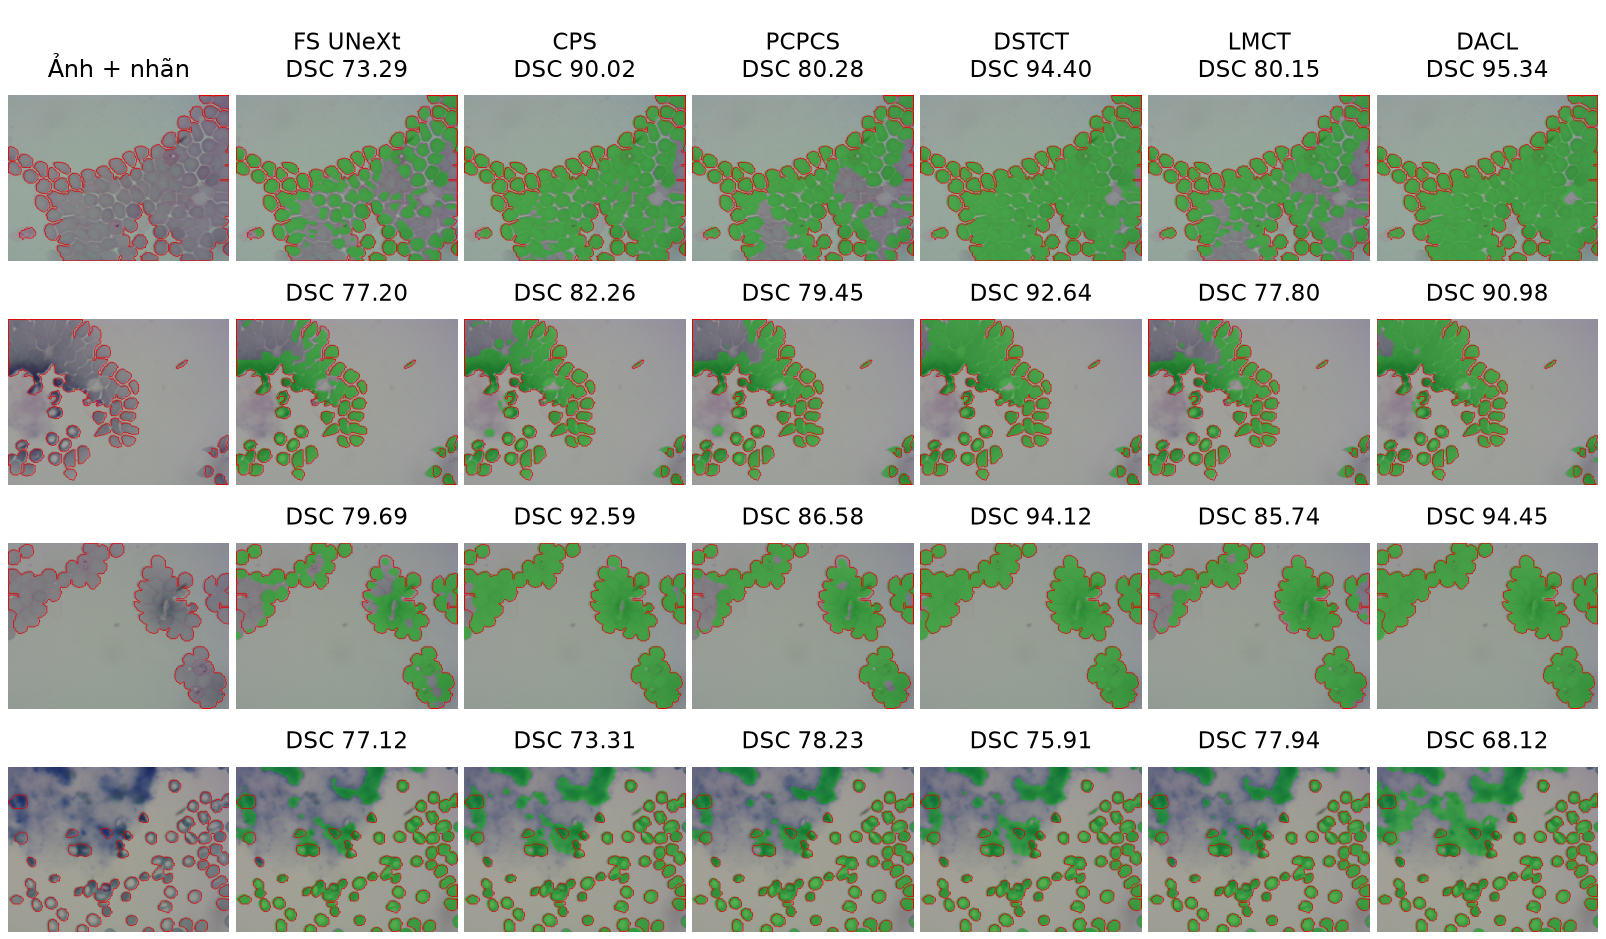
\includegraphics[width=\textwidth]{qualitative_5p.png}
  \caption{Kết quả phân đoạn trên bốn ảnh kiểm thử ở mức 5\% nhãn. Vùng tô xanh: dự đoán. Đường viền đỏ: mặt nạ chuẩn. Số trên mỗi ô là DSC (\%) của ảnh đó. Ảnh được chọn là bốn ảnh có độ lệch chuẩn DSC giữa các mô hình lớn nhất.}
  \label{fig:qual}
\end{figure}

Ba ảnh đầu có chung đặc điểm: tế bào xếp thành cụm dày đặc hoặc chạm nhau thành mảng lớn. UNeXt học có giám sát bỏ sót phần lớn bên trong các cụm này (DSC 73--80\%). DACL và DSTCT, hai phương pháp có giáo viên EMA của Swin-Unet, phủ gần trọn các cụm và đạt DSC trên 90\%. CPS cũng cải thiện đáng kể, còn PCPCS và LMCT cải thiện ít hơn. Ảnh thứ tư cho thấy trường hợp ngược lại. Góc trên bên trái của ảnh có một mảng bắt màu xanh đậm không phải tế bào, và mọi mô hình đều dự đoán nhầm một phần mảng này. DACL nhầm nhiều nhất, với DSC 68,12\%, thấp nhất trong sáu mô hình. Trường hợp này phù hợp với HD95 kém của DACL ở mục~\ref{sec:res-rq1}. Tuy nhiên, nó không đại diện cho toàn bộ tập kiểm thử, vì precision trung bình của DACL vẫn cao nhất trong nhóm bán giám sát. Bốn ảnh không đủ để khái quát, nên hình này chỉ minh họa cho các xu hướng đã đo bằng số liệu ở mục trước.

\section{Diễn biến huấn luyện của DACL (CH3)}
\label{sec:res-dynamics}

Hình~\ref{fig:curves} trình bày DSC kiểm định của UNeXt theo vòng lặp với DACL, hai phương pháp đối chứng CPS và DSTCT, và UNeXt học có giám sát.

\begin{figure}[ht]
  \centering
  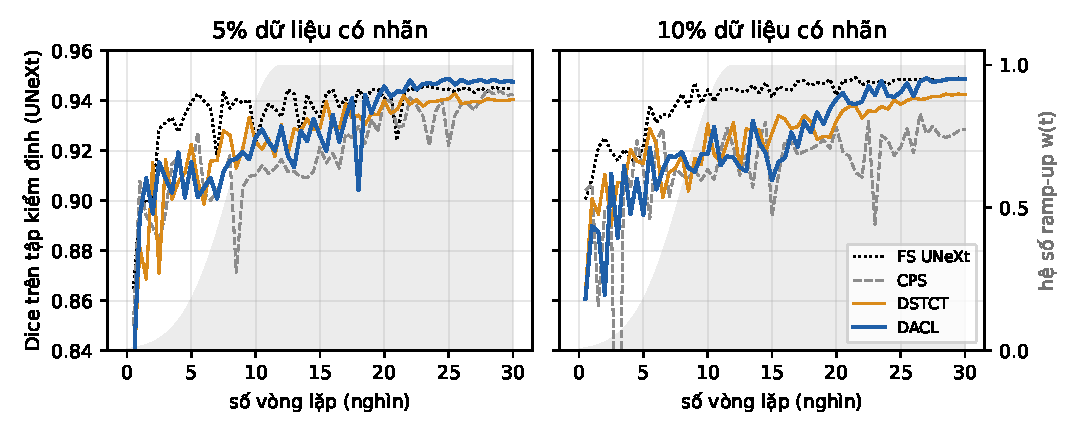
\includegraphics[width=\textwidth]{val_curves.pdf}
  \caption{DSC trên tập kiểm định của UNeXt theo vòng lặp, đo mỗi 500 vòng. Vùng tô xám là hệ số ramp-up $w(t)$ của các phương pháp bán giám sát (trục phải). Trục tung bị cắt ở 0,84.}
  \label{fig:curves}
\end{figure}

Với bộ trọng số $\{0{,}2;\,0{,}2;\,1\}$, DACL huấn luyện ổn định ở cả hai mức nhãn. DSC kiểm định cao nhất đạt 0,9489 ở vòng 25\,000 với 5\% nhãn và 0,9490 ở vòng 27\,000 với 10\% nhãn, đều trong giai đoạn cuối khi tốc độ học đã giảm. Trong 10\,000 vòng cuối, DSC kiểm định của DACL ở mức 5\% có trung bình 0,9467 và độ lệch chuẩn 0,0019. Các giá trị tương ứng của CPS là 0,9370 và 0,0063, của DSTCT là 0,9396 và 0,0017, và của UNeXt học có giám sát là 0,9434 và 0,0045. Ở mức 10\%, DACL đạt 0,9447 với độ lệch chuẩn 0,0036, cao hơn CPS (0,9225; 0,0095) và DSTCT (0,9389; 0,0031) nhưng thấp hơn UNeXt học có giám sát (0,9479; 0,0015). Thứ tự này khớp với kết quả trên tập kiểm thử ở mục~\ref{sec:res-rq1}.

Sau khi hệ số ramp-up đạt giá trị đầy đủ, đường DSC kiểm định của DACL chỉ có hai lần giảm tạm thời: xuống 0,904 ở vòng 18\,000 với 5\% nhãn, và xuống 0,908 ở vòng 15\,000 với 10\% nhãn. Cả hai đều hồi phục ngay ở lần đánh giá kế tiếp, lên 0,942 và 0,915. Log huấn luyện cho thấy, sau vòng 12\,000, phần không giám sát sau khi nhân trọng số chỉ bằng trung bình 18\% phần có giám sát, và không vượt quá 27\% ở cả hai mức nhãn. Như vậy, trong suốt quá trình huấn luyện, tín hiệu giám sát thật vẫn giữ vai trò chủ đạo, đúng như mục tiêu khi lựa chọn trọng số ở mục~\ref{sec:weights}. Hình~\ref{fig:curves} cũng cho thấy UNeXt học có giám sát tăng nhanh hơn hẳn các phương pháp bán giám sát trong 8\,000 vòng đầu, điều sẽ được thảo luận ở Chương~\ref{chap:ketluan}.

\section{Tóm tắt chương}

Chương~\ref{chap:ketqua} đã trình bày kết quả định lượng và định tính cho ba câu hỏi nghiên cứu. Với CH1, DACL có độ trùng khớp cao nhất trong nhóm bán giám sát ở cả hai mức nhãn, nhưng không vượt rõ học có giám sát trên cùng số nhãn và không dẫn đầu về HD95. Với CH2, lợi ích của DACL đến từ việc giảm đồng thời dương tính giả và âm tính giả, và tập trung ở nhóm ảnh khó nhất, đặc biệt là các cụm tế bào dày đặc. Với CH3, DACL huấn luyện ổn định với bộ trọng số đã chọn, và tín hiệu giám sát giữ vai trò chủ đạo trong suốt quá trình huấn luyện. Chương~\ref{chap:ketluan} tóm tắt toàn bộ nghiên cứu, rút ra kết luận cho từng câu hỏi, thảo luận các kết quả trong mối liên hệ với nghiên cứu trước và đưa ra khuyến nghị.
